\documentclass[11pt,a4paper]{article}

\usepackage[T1]{fontenc}
\usepackage{lmodern}
\usepackage[margin=2.3cm]{geometry}
\usepackage{microtype}
\usepackage{amsmath}
\usepackage{booktabs}
\usepackage{tabularx}
\usepackage{longtable}
\usepackage{array}
\usepackage{float}
\usepackage{caption}
\usepackage{enumitem}
\usepackage{xcolor}
\usepackage{tikz}
\usetikzlibrary{positioning,arrows.meta}
\usepackage{pgfplots}
\pgfplotsset{compat=1.18}
\usepackage[colorlinks=true,linkcolor=blue!50!black,urlcolor=blue!50!black,citecolor=blue!50!black]{hyperref}

% chart palette (validated: CVD-safe pair, >= 3:1 contrast on white)
\definecolor{seriesA}{HTML}{2A78D6}
\definecolor{seriesB}{HTML}{EB6834}
\definecolor{inkmuted}{HTML}{52514E}

\captionsetup{font=small,labelfont=bf}
\setlist{itemsep=2pt,topsep=4pt}
\newcolumntype{Y}{>{\raggedright\arraybackslash}X}
\setlength{\emergencystretch}{3em}

\title{\textbf{Hybrid Video Provenance Framework (HVPF)}\\[4pt]
\large Distinguishing Organic, Manipulated and Synthetic Sensor Noise in Digital Videos\\[2pt]
\large Implementation Progress Report}
\author{Talha Aslam\\ MS Thesis}
\date{5 October 2026}

\begin{document}
\maketitle

\begin{abstract}
\noindent This report documents the implementation work carried out so far for the Hybrid Video
Provenance Framework (HVPF) proposed in the thesis. A complete, reproducible nine-step pipeline has
been built: dataset inventory, leakage-free splits, I-frame extraction, PRNU fingerprinting with a
conventional PCE baseline, generation of a manipulated class (PRNU removal, PRNU injection and
denoising attacks), an AI-generated (synthetic) class, feature extraction (PRNU, residual statistics,
FFT, temporal sensor-noise consistency (TSNCS) and Noiseprint++), and classical, deep temporal and
Transformer classifiers with the evaluation protocol of the proposal. Steps 1--6 are complete and
verified; Steps 7--9 are implemented and tested end to end, and the full feature extraction and model
training are running. The PRNU baseline reproduces the expected behaviour on VISION (100\% attribution
of native videos from non-stabilised devices), and several findings relevant to RQ1 and RQ2 have
already emerged. The code is available at
\url{https://github.com/TalhaAslam44/PRNU-Research}.
\end{abstract}

\tableofcontents
\newpage

%=====================================================================
\section{Executive summary}
%=====================================================================

\paragraph{Completed.}
\begin{itemize}
  \item \textbf{Data:} VISION (35 devices, 1{,}914 videos in native, YouTube and WhatsApp versions) and
        Video-ACID (46 devices, 1{,}840 videos streamed from 177\,GB of archives) inventoried and split
        without leakage; 55{,}959 analysis I-frames extracted.
  \item \textbf{Conventional baseline:} per-device PRNU fingerprints and PCE matching for 79 cameras.
  \item \textbf{Manipulated class:} 4{,}400 attacked clips (400 videos $\times$ 11 variants,
        131{,}879 frames) with removal, injection and denoising attacks at several strengths,
        including a white-box removal that drives PCE to zero.
  \item \textbf{Synthetic class:} 1{,}492 AI-generated clips from eight generators (Sora, Kling,
        CogVideo, OpenSora, CogVideoX, EasyAnimate, HunyuanVideo, LTX-Video).
  \item \textbf{Features and models:} all feature extractors (incl.\ GPU Noiseprint++), six model
        families and the full evaluation (PVA, F1, ROC-AUC, EER, ablation) implemented and tested.
\end{itemize}

\paragraph{Key findings so far.}
\begin{enumerate}
  \item Native videos of non-stabilised VISION devices are attributed with 100\% accuracy (AUC 1.000);
        stabilised devices fall to 32\%, confirming that in-camera stabilisation defeats PRNU.
  \item On social-media copies, PCE evaluated at zero shift is far stronger than the usual blind peak
        search (YouTube AUC 0.972 vs 0.812; WhatsApp 0.868 vs 0.713).
  \item Social-media copies of \emph{rotated} recordings lose their PRNU almost entirely (WhatsApp AUC
        0.52 vs 0.92): WhatsApp's rotation path also rescales the video by 0.5--1\% and shifts it by
        3--5 pixels. Geometry, not compression, breaks PRNU here (RQ2).
  \item Video-ACID is bimodal: DSLRs, action cameras and Samsung phones reach 95--100\% attribution,
        while 19 of 44 devices (mostly phones and compact cameras, likely electronically stabilised) show no
        usable video PRNU.
  \item PRNU removal easily over-subtracts: beyond $\alpha\approx0.3$--$0.5$ the PCE becomes strongly
        negative (e.g.\ $-4{,}765$ at $\alpha=1$), itself a detectable trace (RQ1). Injection leaves the true
        camera's fingerprint next to the victim's.
  \item Noiseprint++ does not attribute cameras on luma-only video I-frames (about 20\% top-1 on 10
        cameras), so it is used for output statistics only.
  \item Every clip we re-encode shares an encoder grid that camera originals do not have. An
        \emph{encoder-controlled} evaluation protocol was added so that this cannot inflate the results.
\end{enumerate}

%=====================================================================
\section{Objectives and research questions}
%=====================================================================

The thesis proposes HVPF, a framework that decides whether the sensor noise in a video is
\emph{organic} (produced by a real camera), \emph{manipulated} (suppressed, transferred or injected
by an anti-forensic attack) or \emph{synthetic} (the video is AI-generated). The implementation is
organised around the three research questions:

\begin{description}[leftmargin=1.2cm,style=nextline]
  \item[RQ1] Which characteristics discriminate organic sensor noise from manipulated or synthetic noise?
  \item[RQ2] How do processing operations (compression, resizing, filtering, platform re-encoding)
             affect PRNU-based attribution and noise-based analysis?
  \item[RQ3] Does a hybrid PRNU + machine learning / deep learning framework outperform conventional
             forensic methods for provenance verification and anti-forensic attack detection?
\end{description}

%=====================================================================
\section{System overview}
%=====================================================================

Figure~\ref{fig:pipeline} shows the implemented pipeline. Each step is a separate, resumable script
driven by one configuration file (\texttt{config.yaml}); finished work is skipped on re-runs.

\begin{figure}[H]
\centering
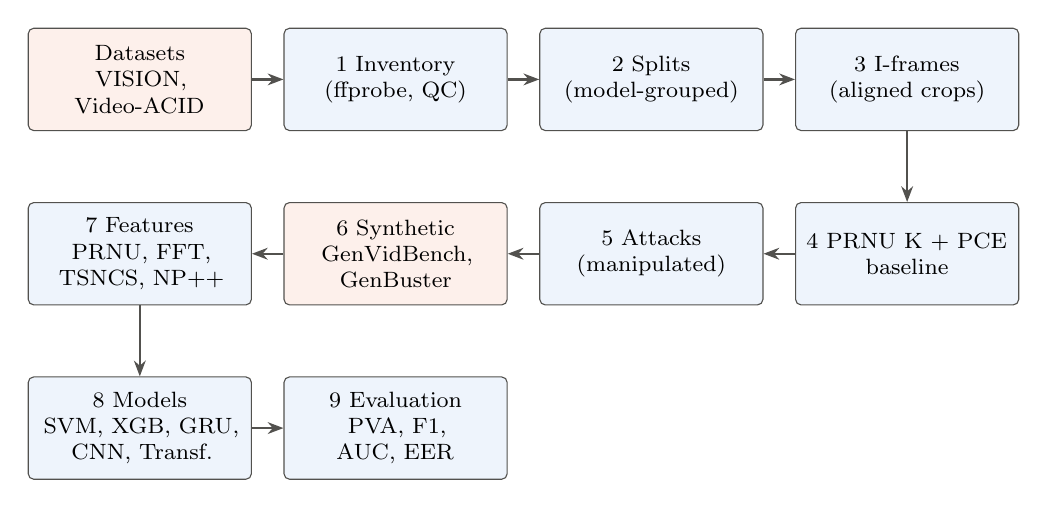
\begin{tikzpicture}[
  node distance=5mm and 4mm,
  box/.style={draw=inkmuted, rounded corners=2pt, align=center, font=\footnotesize,
              minimum height=13mm, text width=26mm, fill=seriesA!8},
  data/.style={box, fill=seriesB!10},
  arr/.style={-{Stealth[length=2mm]}, thick, inkmuted}]
  \node[data] (ds) {Datasets\\VISION, Video-ACID};
  \node[box, right=of ds] (s1) {1 Inventory\\(ffprobe, QC)};
  \node[box, right=of s1] (s2) {2 Splits\\(model-grouped)};
  \node[box, right=of s2] (s3) {3 I-frames\\(aligned crops)};
  \node[box, below=9mm of s3] (s4) {4 PRNU K + PCE\\baseline};
  \node[box, left=of s4] (s5) {5 Attacks\\(manipulated)};
  \node[data, left=of s5] (s6) {6 Synthetic\\GenVidBench, GenBuster};
  \node[box, left=of s6] (s7) {7 Features\\PRNU, FFT, TSNCS, NP++};
  \node[box, below=9mm of s7] (s8) {8 Models\\SVM, XGB, GRU, CNN, Transf.};
  \node[box, right=of s8] (s9) {9 Evaluation\\PVA, F1, AUC, EER};
  \draw[arr] (ds) -- (s1); \draw[arr] (s1) -- (s2); \draw[arr] (s2) -- (s3);
  \draw[arr] (s3) -- (s4); \draw[arr] (s4) -- (s5); \draw[arr] (s5) -- (s6);
  \draw[arr] (s6) -- (s7); \draw[arr] (s7) -- (s8); \draw[arr] (s8) -- (s9);
\end{tikzpicture}
\caption{Implemented HVPF pipeline. Orange boxes are data sources; blue boxes are pipeline steps.}
\label{fig:pipeline}
\end{figure}

\begin{table}[H]
\centering\small
\caption{Implementation environment.}
\begin{tabularx}{\linewidth}{lY}
\toprule
Component & Details \\
\midrule
Hardware & 16-core CPU, 31\,GB RAM, NVIDIA GeForce RTX 3080 (10\,GB, CUDA), spinning hard disk \\
Language and libraries & Python 3.12, PyTorch 2.14 (CUDA), NumPy 2.5, SciPy 1.18, scikit-learn 1.9,
  XGBoost 3.4, OpenCV, pandas 3.0, PyWavelets \\
Video tools & FFmpeg / FFprobe 6.1 (libx264 encoder) \\
PRNU & Politecnico di Milano \texttt{prnu-python}~\cite{prnupython}, patched for NumPy 2 \\
Noiseprint++ & GRIP-UNINA TruFor~\cite{trufor} (nonprofit research licence) \\
Code & \url{https://github.com/TalhaAslam44/PRNU-Research} \\
\bottomrule
\end{tabularx}
\end{table}

%=====================================================================
\section{Datasets}
%=====================================================================

\begin{table}[H]
\centering\small
\caption{Datasets used in the implementation.}
\label{tab:datasets}
\begin{tabularx}{\linewidth}{lYrl}
\toprule
Dataset & Content & Videos & Role \\
\midrule
VISION~\cite{vision} & 35 devices, 11 brands; native videos and their YouTube and WhatsApp copies;
  flat, indoor and outdoor scenes & 1{,}914 & organic, attack source \\
Video-ACID~\cite{acid} & 46 devices of 36 camera models (phones, DSLRs, compacts, camcorders,
  action cameras); first 40 videos per device & 1{,}840 & organic \\
GenVidBench~\cite{genvidbench} & AI-generated: Sora, Kling, CogVideo, OpenSora & 892 & synthetic \\
GenBuster-200K-mini~\cite{busterx} & AI-generated: CogVideoX, EasyAnimate, HunyuanVideo, LTX-Video & 600 &
  unseen-generator test \\
FloreView~\cite{floreview} & 46 smartphones (videos only, about 95\,GB) & -- & pending \\
\bottomrule
\end{tabularx}
\end{table}

\subsection{Inventory and quality control (Step 1)}
Every video was probed with FFprobe (codec, resolution, rotation flag, frame rate, duration, number of
I-frames) and the full packet stream was read to detect truncated files.

\begin{itemize}
  \item \textbf{VISION:} 1{,}914 videos (648 native, 622 YouTube, 644 WhatsApp), all H.264.
        One file is truncated (\texttt{D33\_V\_indoorYT\_panrot\_0001.mp4}, ``moov atom not found'')
        and six videos listed as misplaced in the VISION errata are excluded.
        About 1 I-frame per second (median 70 per native video); YouTube copies have about 15.
  \item \textbf{Stabilisation:} 14 VISION devices use in-camera digital stabilisation
        (D02, D05, D06, D10, D12, D14, D15, D18, D19, D20, D25, D29, D32, D34), following the VISION
        paper and Mandelli et al.~\cite{mandelli}. They are kept and reported separately.
  \item \textbf{Video-ACID:} the archives (177\,GB) exceed the free disk space, so they are streamed:
        the first 40 videos of each device are kept, probed and reduced to I-frames, and the videos are
        deleted. ACID clips are short (median 5--7\,s, about 6 I-frames). The Nokia 6.1 (2 devices,
        80 videos) uses an MP4 feature FFmpeg 6.1 cannot read and is excluded.
  \item \textbf{Resolution:} two VISION devices record at 800$\times$480 (D04) and 640$\times$480 (D23),
        which fixed the analysis crop at 480$\times$480 (the proposal suggested 512$\times$512).
\end{itemize}
The per-device table for VISION (the planned Chapter~5 table) is given in Appendix~\ref{app:vision}.

%=====================================================================
\section{Experimental protocol (Step 2)}
%=====================================================================

\paragraph{Device- and model-disjoint splits.} The split unit is the \emph{camera model}: all devices
of one model (e.g.\ the three iPhone~5c units D05, D14, D18) are kept in the same split, and VISION and
ACID devices of the same phone model (e.g.\ Galaxy S5) are grouped across datasets. This is stricter
than the device split of the plan, because Noiseprint is a model-level trace. Every version of a
recording (native, YouTube, WhatsApp and later the attacked copies) inherits its device's split.
Groups are dealt 60/20/20 within strata (dataset mix $\times$ stabilisation). Assertions verify that no
device, model or recording crosses splits.

\paragraph{Cross-validation.} With 35 VISION devices a single test split holds only five cameras, so
a 5-fold grouped assignment is also produced; results will be reported as mean $\pm$ standard
deviation over folds, with the fixed split as a secondary view.

\begin{table}[H]
\centering\small
\caption{VISION devices per split and per fold (stabilised devices in brackets).}
\begin{tabularx}{\linewidth}{lY}
\toprule
Split / fold & Devices \\
\midrule
Train (22) & D01 [D02] D03 [D05] D08 D09 [D10] D13 [D14] D17 [D18] D24 [D25] D26 D27 D28 [D29] D30 D31 [D32] [D34] D35 \\
Validation (8) & D04 [D06] D11 [D15] D16 [D20] D22 D33 \\
Test (5) & D07 [D12] [D19] D21 D23 \\
\midrule
Fold 0 & D01 D07 D09 [D20] [D25] D26 D27 D30 [D32] \\
Fold 1 & [D05] D08 D11 D13 [D14] [D18] D28 D33 \\
Fold 2 & D03 [D06] [D15] D16 [D19] D23 D35 \\
Fold 3 & [D02] D04 [D10] [D12] D22 D24 \\
Fold 4 & D17 D21 [D29] D31 [D34] \\
\bottomrule
\end{tabularx}
\end{table}
ACID devices are split in the same way (27 train, 11 validation, 8 test).

\paragraph{Roles.} VISION native \emph{flat} videos are \emph{reference} videos that estimate each
camera's fingerprint; their YouTube/WhatsApp copies are not used, so the reference never leaks into
evaluation. Natural (indoor/outdoor) videos in all versions are \emph{samples}. ACID has no flat
videos: the first 20 videos of each device are references and the next 20 are samples.

%=====================================================================
\section{Frame extraction (Step 3)}
%=====================================================================

Up to 30 I-frames per video (evenly spaced over all I-frames) are decoded, converted to luma and
center-cropped to 480$\times$480. Because PRNU is a pixel-wise pattern, frames are kept in the
\emph{sensor} orientation: videos are decoded without applying their rotation flag. YouTube and
WhatsApp copies bake the rotation into the pixels and are downscaled (e.g.\ WhatsApp stores 848$\times$480
or 480$\times$848), so they are rotated back and rescaled to the native resolution before cropping.
A content check confirmed the alignment (correlation 0.95--0.997 between native and aligned
WhatsApp frames). Result: 1{,}480 VISION videos (39{,}404 frames, median 30 per video) and 1{,}760 ACID
videos (16{,}555 frames, median 7).

%=====================================================================
\section{PRNU fingerprints and conventional baseline (Step 4)}
%=====================================================================

\subsection{Method}
For each camera the maximum-likelihood fingerprint
$\hat K = \sum_i W_i I_i / \sum_i I_i^2$~\cite{chen2008} is estimated from its reference frames,
where $W_i$ is the wavelet-denoised residual of frame $I_i$. The Politecnico di Milano
implementation~\cite{prnupython} was used; it needed two fixes (a NumPy~2 incompatibility, and
its multi-image estimator only handled RGB), and the grayscale estimator matches the original to
$6\times10^{-7}$. Each sample video gets its own fingerprint from its I-frames, which is compared
with every camera of the dataset by:
\begin{itemize}
  \item \textbf{PCE (blind):} peak-to-correlation energy with the peak searched over all shifts~\cite{lukas2006};
  \item \textbf{PCE$_0$:} PCE evaluated at zero shift, since our frames are aligned by construction;
  \item \textbf{NCC:} normalised correlation at zero shift.
\end{itemize}
Closed-set attribution picks the camera with the highest score; verification uses the common
threshold PCE\,$>$\,60.

\subsection{VISION results}

\begin{table}[H]
\centering\small
\caption{PRNU baseline on VISION (35 cameras, closed set). Accuracy = closed-set attribution;
AUC and EER for verification of matching vs non-matching camera pairs.}
\label{tab:vision}
\begin{tabular}{llrrrrrr}
\toprule
Version & Devices & Queries & Acc.\ PCE$_0$ & AUC PCE$_0$ & AUC PCE & EER PCE$_0$ & TPR@60 \\
\midrule
Native   & non-stabilised & 259 & 100.0\% & 1.000 & 0.999 & 0.000 & 0.954 \\
Native   & stabilised     & 166 &  31.9\% & 0.738 & 0.564 & 0.344 & 0.145 \\
YouTube  & non-stabilised & 249 &  84.7\% & 0.972 & 0.812 & 0.084 & 0.257 \\
YouTube  & stabilised     & 162 &  20.4\% & 0.638 & 0.489 & 0.437 & 0.031 \\
WhatsApp & non-stabilised & 257 &  60.7\% & 0.868 & 0.713 & 0.214 & 0.257 \\
WhatsApp & stabilised     & 166 &   7.8\% & 0.571 & 0.464 & 0.453 & 0.006 \\
\bottomrule
\end{tabular}
\end{table}

\begin{figure}[H]
\centering
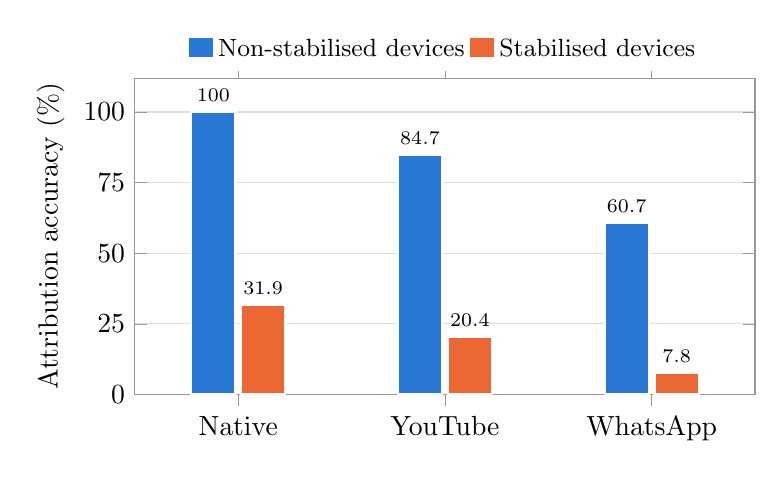
\begin{tikzpicture}
\begin{axis}[
  ybar, bar width=16pt, width=0.78\linewidth, height=5.6cm,
  ymin=0, ymax=112, ytick={0,25,50,75,100},
  symbolic x coords={Native,YouTube,WhatsApp}, xtick=data, enlarge x limits=0.25,
  ylabel={Attribution accuracy (\%)}, ymajorgrids, grid style={draw=black!12},
  axis line style={draw=black!40}, tick style={draw=black!40},
  nodes near coords, nodes near coords style={font=\scriptsize, text=black},
  every node near coord/.append style={/pgf/number format/.cd, fixed, precision=1},
  legend style={at={(0.5,1.02)}, anchor=south, legend columns=-1, draw=none, font=\small},
  legend image code/.code={\draw[#1, draw=none] (0cm,-0.1cm) rectangle (0.3cm,0.15cm);}]
\addplot[fill=seriesA, draw=white, line width=0.8pt] coordinates {(Native,100.0) (YouTube,84.7) (WhatsApp,60.7)};
\addplot[fill=seriesB, draw=white, line width=0.8pt] coordinates {(Native,31.9) (YouTube,20.4) (WhatsApp,7.8)};
\legend{Non-stabilised devices, Stabilised devices}
\end{axis}
\end{tikzpicture}
\caption{Closed-set attribution (PCE$_0$) on VISION by version.}
\label{fig:vision}
\end{figure}

\paragraph{Observations.}
Native videos of non-stabilised devices are attributed perfectly, consistent with published results
on VISION~\cite{vision}; digital stabilisation breaks PRNU, as reported in~\cite{mandelli}. On
social-media copies PCE$_0$ is clearly better than the blind peak search, so PCE$_0$ is used as the
conventional method for RQ3. The fixed threshold of 60 is very conservative for social copies
(true-positive rate about 0.26 at zero false positives).

\subsection{Rotation finding (RQ2)}
Breaking the non-stabilised results down by whether the original recording carried a rotation flag
reveals a strong effect on social-media copies (Table~\ref{tab:rotation}).

\begin{table}[H]
\centering\small
\caption{Non-stabilised VISION devices: effect of the original recording's rotation flag.}
\label{tab:rotation}
\begin{tabular}{llrrr}
\toprule
Version & Original rotated & Queries & Acc.\ PCE$_0$ & AUC PCE$_0$ \\
\midrule
Native   & no  & 225 & 100.0\% & 1.000 \\
Native   & yes &  34 & 100.0\% & 1.000 \\
YouTube  & no  & 222 &  88.3\% & 0.982 \\
YouTube  & yes &  27 &  55.6\% & 0.896 \\
WhatsApp & no  & 223 &  70.0\% & 0.920 \\
WhatsApp & yes &  34 &   0.0\% & 0.523 \\
\bottomrule
\end{tabular}
\end{table}

Native rotated videos are unaffected, so the geometric inversion is correct. Phase correlation
between native and WhatsApp frames showed that WhatsApp copies of rotated recordings are offset by
3--5 pixels (versus 0.35 pixels for unrotated ones) and an affine registration found an extra scaling
of 0.5--1\%. Registering the frames to the native video restored the match (e.g.\ PCE from 44 to 213).
Hence a platform's handling of rotation, not its compression, removes the PRNU in these copies; a blind
analyst would need a scale search to recover it.

\subsection{Video-ACID results}
ACID is much harder: 50.7\% closed-set attribution (PCE$_0$, 44 cameras) and AUC 0.80, because there
are no flat videos (fingerprints come from about 120 natural frames per camera) and many 2017--18
devices stabilise electronically. Per device the result is bimodal (Figure~\ref{fig:acid}).

\begin{figure}[H]
\centering
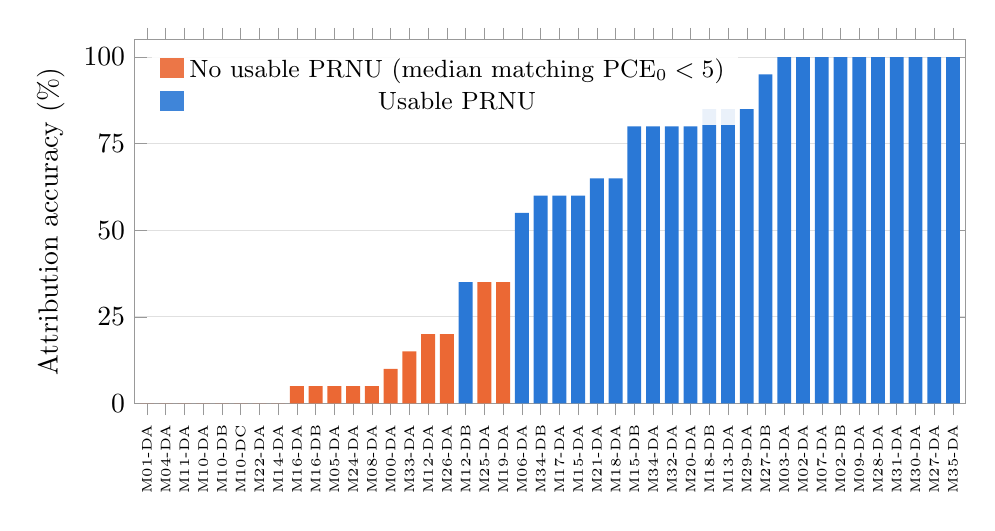
\begin{tikzpicture}
\begin{axis}[
  ybar, bar width=5pt, bar shift=0pt, width=\linewidth, height=6.2cm,
  ymin=0, ymax=105, ytick={0,25,50,75,100},
  symbolic x coords={M01-DA,M04-DA,M11-DA,M10-DA,M10-DB,M10-DC,M22-DA,M14-DA,M16-DA,M16-DB,M05-DA,M24-DA,M08-DA,M00-DA,M33-DA,M12-DA,M26-DA,M12-DB,M25-DA,M19-DA,M06-DA,M34-DB,M17-DA,M15-DA,M21-DA,M18-DA,M15-DB,M34-DA,M32-DA,M20-DA,M18-DB,M13-DA,M29-DA,M27-DB,M03-DA,M02-DA,M07-DA,M02-DB,M09-DA,M28-DA,M31-DA,M30-DA,M27-DA,M35-DA},
  xtick={M01-DA,M04-DA,M11-DA,M10-DA,M10-DB,M10-DC,M22-DA,M14-DA,M16-DA,M16-DB,M05-DA,M24-DA,M08-DA,M00-DA,M33-DA,M12-DA,M26-DA,M12-DB,M25-DA,M19-DA,M06-DA,M34-DB,M17-DA,M15-DA,M21-DA,M18-DA,M15-DB,M34-DA,M32-DA,M20-DA,M18-DB,M13-DA,M29-DA,M27-DB,M03-DA,M02-DA,M07-DA,M02-DB,M09-DA,M28-DA,M31-DA,M30-DA,M27-DA,M35-DA}, x tick label style={rotate=90, font=\tiny, anchor=east},
  enlarge x limits=0.015, ylabel={Attribution accuracy (\%)},
  ymajorgrids, grid style={draw=black!12}, axis line style={draw=black!40}, tick style={draw=black!40},
  legend style={at={(0.02,0.98)}, anchor=north west, draw=none, font=\small, fill=white, fill opacity=0.9, text opacity=1},
  legend image code/.code={\draw[#1, draw=none] (0cm,-0.1cm) rectangle (0.3cm,0.15cm);}]
\addplot[fill=seriesB, draw=none] coordinates {
 (M01-DA,0) (M04-DA,0) (M11-DA,0) (M10-DA,0) (M10-DB,0) (M10-DC,0) (M22-DA,0) (M14-DA,0)
 (M16-DA,5) (M16-DB,5) (M05-DA,5) (M24-DA,5) (M08-DA,5) (M00-DA,10) (M33-DA,15) (M12-DA,20)
 (M26-DA,20) (M25-DA,35) (M19-DA,35)};
\addplot[fill=seriesA, draw=none] coordinates {
 (M12-DB,35) (M06-DA,55) (M34-DB,60) (M17-DA,60) (M15-DA,60) (M21-DA,65) (M18-DA,65) (M15-DB,80)
 (M34-DA,80) (M32-DA,80) (M20-DA,80) (M18-DB,85) (M13-DA,85) (M29-DA,85) (M27-DB,95) (M03-DA,100)
 (M02-DA,100) (M07-DA,100) (M02-DB,100) (M09-DA,100) (M28-DA,100) (M31-DA,100) (M30-DA,100)
 (M27-DA,100) (M35-DA,100)};
\legend{No usable PRNU (median matching PCE$_0<5$), Usable PRNU}
\end{axis}
\end{tikzpicture}
\caption{Per-device attribution on Video-ACID (20 sample videos per device), sorted. Devices are
ACID model ids (e.g.\ M10 = Google Pixel 1, M00 = iPhone 8 Plus, M35 = Yi 4K action camera).}
\label{fig:acid}
\end{figure}

DSLRs (Canon EOS SL1/T6i), action cameras (GoPro, Yi 4K) and most Samsung phones reach 95--100\% with
matching PCE in the hundreds to thousands, whereas 19 devices (Google Pixel 1 and 2, iPhone~8 Plus,
LG Q6, Asus Zenfone~3, several compact cameras and camcorders) have a
median matching PCE below 5, most likely because of electronic image stabilisation. They are flagged as \emph{PRNU-weak} for the analysis; the splits are
unchanged.

%=====================================================================
\section{Manipulated class (Step 5)}
%=====================================================================

\subsection{Attack design}
The targets are the 400 natural native VISION videos (up to 12 per device). The first 30\,s of each
are decoded once in sensor orientation, cropped like the analysis frames, attacked on the luma
channel only, and re-encoded with libx264 (CRF 20, one I-frame per second, about 30 I-frames per
clip, matching the organic samples). Table~\ref{tab:attacks} lists the 11 variants per target.

\begin{table}[H]
\centering\small
\caption{Variants generated per target video. $\alpha$ is in units of a 1\% PRNU: attacker
fingerprints are rescaled to standard deviation 0.01.}
\label{tab:attacks}
\begin{tabularx}{\linewidth}{lYll}
\toprule
Variant & Operation & Label & Claimed camera \\
\midrule
\texttt{reencode} & same encoder, no attack (control) & organic & own \\
\texttt{removal}, $\alpha\in\{0.25,0.5,1\}$ & $F' = F - \alpha F \hat K_{\text{own}}$ & manipulated & own \\
\texttt{removal\_opt} & white-box: $\alpha$ tuned per clip until NCC with the analyst's reference is $\approx 0$ & manipulated & own \\
\texttt{injection}, $\alpha\in\{0.25,0.5,1\}$ & $F' = F + \alpha F \hat K_{\text{victim}}$ (fingerprint-copy attack~\cite{goljan2011}) & manipulated & victim \\
\texttt{denoise}, $s\in\{1,2,4\}$ & hqdn3d denoising at $s\times$ default strength (desynchronisation) & manipulated & own \\
\bottomrule
\end{tabularx}
\end{table}

\paragraph{Attacker knowledge.} The attacker never uses the analyst's flat-field reference.
$\hat K_{\text{own}}$ is estimated from the \emph{other half} of the device's natural videos, and
$\hat K_{\text{victim}}$ from all natural videos of a non-stabilised victim of another camera model in the
same cross-validation fold (so no test camera enters training). The white-box removal is the
deliberate exception: it represents the worst case for the PCE baseline. A natural-video-only
calibration was tried first but gave values of $\alpha$ about five times too small: VISION films each
device's natural videos at the same places, so two natural-video fingerprint estimates share scene
residue. The white-box attacker therefore calibrates $\alpha$ by secant steps on the analyst's own
measurement (median $\alpha^\ast = 0.39$, interquartile range 0.24--0.57).

\paragraph{Control.} The \texttt{reencode} clips pass through exactly the same encoder as the attacks
and are labelled organic, so encoder traces alone cannot separate the classes.

\subsection{Verification}
Table~\ref{tab:attackcheck} shows PCE$_0$ against the analyst's references for two test videos.

\begin{table}[H]
\centering\small\setlength{\tabcolsep}{4.5pt}
\caption{PCE$_0$ of attacked clips against the analyst's references (own camera / injected victim).}
\label{tab:attackcheck}
\begin{tabular}{lrrrr}
\toprule
& \multicolumn{2}{c}{D01 (victim D30)} & \multicolumn{2}{c}{D08 (victim D28)} \\
\cmidrule(lr){2-3}\cmidrule(lr){4-5}
Variant & own & victim & own & victim \\
\midrule
Original native        & 563   & 1    & 2{,}771  & 0 \\
\texttt{reencode}      & 195   & 0    & 1{,}381  & 1 \\
\texttt{removal} 0.25 / 0.5 / 1 & 12 / $-199$ / $-1{,}296$ & -- & 644 / 3 / $-4{,}765$ & -- \\
\texttt{removal\_opt}  & 0.1 ($\alpha^\ast$=0.30) & -- & 0.0 ($\alpha^\ast$=0.52) & -- \\
\texttt{injection} 0.25 / 0.5 / 1 & 146 / 91 / 18 & 49 / 315 / 919 & 1{,}343 / 1{,}185 / 582 & 39 / 275 / 1{,}357 \\
\texttt{denoise} 1 / 2 / 4 & 103 / 75 / 38 & -- & 1{,}124 / 918 / 454 & -- \\
\bottomrule
\end{tabular}
\end{table}

All variants behave as intended: injection makes the victim match while the true camera remains
detectable; removal over-subtracts quickly and leaves a strongly \emph{negative} PCE, a trace that a
classifier can learn; the white-box removal lands at PCE$\approx0$, the hardest case for the baseline.
Output: 4{,}400 clips and 131{,}879 frames with no failures.

%=====================================================================
\section{Synthetic class (Step 6)}
%=====================================================================

\begin{table}[H]
\centering\small
\caption{AI-generated clips used (after quality checks). Frames = median I-frames per clip.}
\label{tab:synthetic}
\begin{tabular}{llrrrrrr}
\toprule
Source & Generator & Native format & Frames & Train & Val & Test & Unseen test \\
\midrule
GenVidBench & Sora     & 1080p, $\sim$17\,s & 18 & 26  & 17 & 8  & -- \\
            & Kling    & 720p, 5--10\,s     & 6  & 151 & 74 & 44 & -- \\
            & CogVideo & 480$\times$480, 4\,s & 5 & 166 & 76 & 58 & -- \\
            & OpenSora & 512$\times$512, 2\,s & 2 & 141 & 89 & 42 & -- \\
GenBuster   & 4 generators$^{a}$ & 1024$^2$ HEVC, 5\,s & 6 & -- & -- & -- & 4 $\times$ 150 \\
\midrule
Total       & & & & 484 & 256 & 152 & 600 \\
\bottomrule
\multicolumn{8}{l}{\footnotesize $^{a}$\,CogVideoX, EasyAnimate, HunyuanVideo and LTX-Video, 150 clips each.}
\end{tabular}
\end{table}

Generator files contain almost no I-frames (e.g.\ one per Kling clip), so the synthetic clips go
through the same libx264 pipeline as the attacks and the control (one I-frame per second, same crop).
Frame type, spacing and encoder are therefore identical across classes. Denser sampling of short
clips was rejected, because frames closer in time inflate TSNCS and would create a false
``synthetic'' cue. Each clip claims a random camera (VISION or ACID) of a random fold, so the PRNU
features can be computed; its split follows that camera. GenBuster is held out as an unseen-generator
test set; its real videos are not used because they have no camera reference.

%=====================================================================
\section{Feature extraction (Step 7)}
%=====================================================================

\begin{table}[H]
\centering\small
\caption{Feature groups. Per-frame values are aggregated (mean, standard deviation) per clip.}
\label{tab:features}
\begin{tabularx}{\linewidth}{lY}
\toprule
Group & Features \\
\midrule
PRNU & per frame: NCC and PCE$_0$ between the residual $W$ and $I\hat K$ of the claimed camera;
       per clip: PCE, PCE$_0$ and NCC of the clip fingerprint with the claimed camera, and the best
       match among all \emph{other} known cameras (injection leaves a second fingerprint) \\
Residual & standard deviation, skewness and kurtosis of the noise residual \\
FFT & spectral flatness, high-frequency energy share, peak ratio, number of periodic peaks, 8-pixel
      block-grid energy of the residual spectrum \\
TSNCS & normalised correlation between residuals of consecutive I-frames (mean, std, minimum) \\
Noiseprint++ & map std and kurtosis, FFT statistics of the map, spectral similarity to the claimed
      camera's reference (GPU) \\
\bottomrule
\end{tabularx}
\end{table}

\paragraph{Fixed-length windows.} Clips differ in length (VISION about 30 I-frames, ACID about 6,
synthetic 2--20). All model inputs are therefore computed from the \emph{first five} I-frames of every
clip, so clip length cannot act as a shortcut.

\paragraph{Noiseprint++.} Noiseprint++, the pretrained extractor of TruFor~\cite{trufor} and successor of
Noiseprint~\cite{noiseprint}, runs on the GPU. In a test on 10 VISION cameras its maps did not
attribute cameras: 20\% top-1 with spatial similarity and 17.5\% (25\% at model level) with spectral
similarity, against 10\% chance. It was trained on RGB still images, whereas our frames are luma-only,
heavily compressed video I-frames. Its output statistics are kept as a feature group, and the
ablation will quantify their contribution.

\paragraph{Encoder confound and the controlled protocol.} The Noiseprint 8-pixel grid energy is about
4 for every clip we encode with libx264 and about 0.65 for organic WhatsApp clips: our encodes start
their macroblock grid at the crop origin, camera originals do not. To prevent a classifier from
exploiting this, results will be reported under two protocols:
\begin{itemize}
  \item \textbf{Realistic:} all organic samples vs manipulated and synthetic;
  \item \textbf{Encoder-controlled:} only libx264 clips (\texttt{reencode} controls vs attacks vs
        synthetic), where encoder and grid are identical across classes.
\end{itemize}

\paragraph{Preliminary check.} On a random check set of 100 samples, the median clip PCE$_0$ with the
claimed camera was 20.7 for organic, 61.9 for manipulated (inflated by injection) and 0.07 for
synthetic clips, and the median TSNCS was 0.001, 0.003 and 0.019 respectively; on test clips TSNCS
rose from about 0.002 at removal strength $\alpha=0.25$ to 0.17 at $\alpha=1$. These numbers only confirm that the extractors work; the full
extraction over all 8{,}031 samples (2{,}539 organic, 4{,}000 manipulated, 1{,}492 synthetic) is running.

%=====================================================================
\section{Models and evaluation (Steps 8--9)}
%=====================================================================

\begin{itemize}
  \item \textbf{Conventional baseline:} organic if PCE$_0$ with the claimed camera exceeds 60 (binary
        decision; it cannot tell manipulated from synthetic).
  \item \textbf{Classical ML:} SVM (RBF kernel, $C$ chosen on validation) and XGBoost (depth chosen on
        validation, early stopping) on the clip-level features.
  \item \textbf{Deep temporal:} GRU and 1D-CNN on the per-frame feature sequences, pooled and joined
        with the clip-level features.
  \item \textbf{Transformer:} a two-layer Transformer encoder on the same sequences, as in the proposal.
\end{itemize}
Networks use Adam (learning rate 0.001), L2 weight decay ($10^{-4}$), a class-balanced cross-entropy
loss and early stopping on validation macro-F1. Every configuration is run under both protocols and
both schemes (fixed split and 5-fold cross-validation), with GenBuster as the unseen-generator test.

\paragraph{Metrics.} PVA (the share of videos assigned to their true provenance category, i.e.\
3-class accuracy, as defined in the proposal), macro precision, recall and F1, one-vs-rest ROC-AUC,
and ROC-AUC and EER for authentic versus non-authentic (where the PCE baseline is compared, RQ3).
For RQ2 the detection rate is broken down by version (native, YouTube, WhatsApp), attack type and
strength $\alpha$, generator, and stabilisation. The ablation removes one feature group at a time
(PRNU, residual, FFT, TSNCS, Noiseprint), with special attention to TSNCS.

\paragraph{Status.} All model and evaluation code has been tested end to end on a check set. The full
runs (14 configurations) start automatically once the feature extraction finishes.

%=====================================================================
\section{Deviations from the proposal}
%=====================================================================

\begin{table}[H]
\centering\small
\caption{Changes with respect to the thesis proposal and their justification.}
\begin{tabularx}{\linewidth}{lYY}
\toprule
Aspect & Proposal & Implementation and reason \\
\midrule
Datasets & PRNU-Bench, VISION, Dresden & VISION, Video-ACID, GenVidBench, GenBuster, FloreView (pending):
  PRNU-Bench and Dresden are image datasets; the thesis is about video \\
Split & random 80:10:10 & model-grouped 60/20/20 plus 5-fold CV: test cameras (and camera models)
  must never be seen in training, and 35 devices are too few for one small test split \\
Crop & 512$\times$512 suggested & 480$\times$480: two VISION devices record 480 pixels high \\
Classifier & Transformer & PCE baseline, SVM, XGBoost, GRU, 1D-CNN and Transformer, to answer RQ3 \\
Noiseprint & similarity to a reference & output statistics plus spectral similarity, since attribution
  with Noiseprint++ is weak on our frames \\
Evaluation & one protocol & realistic and encoder-controlled protocols (encoder confound) \\
\bottomrule
\end{tabularx}
\end{table}

%=====================================================================
\section{Technical issues and resolutions}
%=====================================================================

\begin{table}[H]
\centering\small
\begin{tabularx}{\linewidth}{YY}
\toprule
Issue & Resolution \\
\midrule
Only about 50\,GB free disk for 280\,GB of video data & ACID streamed from its archives; frames of
  attacks and synthetic clips stored on a second partition \\
GPU unavailable (NVIDIA driver not loaded) & resolved after a reboot; CUDA verified on the RTX 3080 \\
PRNU library incompatible with NumPy 2, RGB-only estimator & minimal patch (kept as a patch file);
  grayscale estimator added and verified against the original \\
Platform copies rotated and rescaled & rotation undone and frames rescaled to native geometry;
  residual misalignment of rotated WhatsApp copies analysed (RQ2) \\
Camcorder \texttt{.MTS} files and unreadable Nokia MP4 files in ACID & \texttt{.MTS} supported;
  Nokia 6.1 excluded and documented \\
Attack strength calibration & $\alpha$ grid plus a white-box attacker calibrated on the analyst's
  measurement \\
Clip length and encoder differences between classes & fixed five-frame windows; shared libx264
  pipeline with organic re-encode controls; encoder-controlled protocol \\
\bottomrule
\end{tabularx}
\end{table}

%=====================================================================
\section{Current status and next steps}
%=====================================================================

\begin{table}[H]
\centering\small
\begin{tabularx}{\linewidth}{lYl}
\toprule
Step & Content & Status \\
\midrule
1 & Inventory and quality control & done \\
2 & Splits and folds & done \\
3 & I-frame extraction & done \\
4 & PRNU fingerprints and PCE baseline & done (VISION, ACID) \\
5 & Manipulated class & done (4{,}400 clips) \\
6 & Synthetic class & done (1{,}492 clips) \\
7 & Feature extraction (incl.\ Noiseprint++) & implemented; full run in progress \\
8 & Models & implemented and tested; queued \\
9 & Evaluation and ablation & implemented and tested; queued \\
\bottomrule
\end{tabularx}
\end{table}

\paragraph{Next steps.}
\begin{enumerate}
  \item Analyse the model results: per-class performance, comparison with the PCE baseline (RQ3),
        detection rate per version and attack strength (RQ2), and feature importance and ablation (RQ1).
  \item Add FloreView as the cross-dataset test for organic videos (download in progress).
  \item Optionally test robustness of the detectors when attacked clips are themselves shared through
        a social-media-like re-encoding.
  \item Write the results and discussion chapters.
\end{enumerate}

\paragraph{Points for discussion with the supervisor.}
\begin{itemize}
  \item Approval of the dataset change (video datasets instead of PRNU-Bench and Dresden) and of the
        model-grouped split with 5-fold cross-validation.
  \item Whether the encoder-controlled protocol should be the primary result.
  \item Whether to re-extract RGB frames to give Noiseprint++ a fair chance, at a substantial cost in
        time and storage.
  \item Scope of the FloreView cross-dataset experiment.
\end{itemize}

%=====================================================================
\begin{thebibliography}{99}
\bibitem{vision} D.~Shullani, M.~Fontani, M.~Iuliani, O.~Al~Shaya, A.~Piva,
  ``VISION: a video and image dataset for source identification,''
  \emph{EURASIP Journal on Information Security}, 2017.
\bibitem{acid} B.~Hosler, O.~Mayer, B.~Bayar, X.~Zhao, C.~Chen, J.~A.~Shackleford, M.~C.~Stamm,
  ``A video camera model identification system using deep learning and fusion,''
  \emph{IEEE ICASSP}, 2019 (Video-ACID dataset).
\bibitem{floreview} D.~Baracchi, D.~Shullani, M.~Iuliani, A.~Piva,
  ``FloreView: an image and video dataset for forensic analysis,'' \emph{IEEE Access}, 2023.
\bibitem{genvidbench} ``GenVidBench: A 6-million benchmark for AI-generated video detection,''
  \emph{AAAI}, 2026, arXiv:2501.11340.
\bibitem{busterx} ``BusterX: MLLM-powered AI-generated video forgery detection and explanation,''
  arXiv:2505.12620, 2025 (GenBuster-200K dataset).
\bibitem{lukas2006} J.~Luk\'a\v{s}, J.~Fridrich, M.~Goljan,
  ``Digital camera identification from sensor pattern noise,''
  \emph{IEEE Trans.\ Information Forensics and Security}, 2006.
\bibitem{chen2008} M.~Chen, J.~Fridrich, M.~Goljan, J.~Luk\'a\v{s},
  ``Determining image origin and integrity using sensor noise,''
  \emph{IEEE Trans.\ Information Forensics and Security}, 2008.
\bibitem{goljan2011} M.~Goljan, J.~Fridrich, M.~Chen,
  ``Defending against fingerprint-copy attack in sensor-based camera identification,''
  \emph{IEEE Trans.\ Information Forensics and Security}, 2011.
\bibitem{mandelli} S.~Mandelli, P.~Bestagini, L.~Verdoliva, S.~Tubaro,
  ``Facing device attribution problem for stabilized video sequences,''
  \emph{IEEE Trans.\ Information Forensics and Security}, 2020.
\bibitem{noiseprint} D.~Cozzolino, L.~Verdoliva,
  ``Noiseprint: a CNN-based camera model fingerprint,''
  \emph{IEEE Trans.\ Information Forensics and Security}, 2020.
\bibitem{trufor} F.~Guillaro, D.~Cozzolino, A.~Sud, N.~Dufour, L.~Verdoliva,
  ``TruFor: leveraging all-round clues for trustworthy image forgery detection and localization,''
  \emph{IEEE/CVF CVPR}, 2023.
\bibitem{prnupython} L.~Bondi, P.~Bestagini, N.~Bonettini,
  ``prnu-python: Python porting of the PRNU extractor,'' Politecnico di Milano,
  \url{https://github.com/polimi-ispl/prnu-python}.
\end{thebibliography}

%=====================================================================
\appendix
\section{VISION devices}
\label{app:vision}
%=====================================================================

{\small
\setlength{\tabcolsep}{4pt}
\begin{longtable}{lllllrrrrlr}
\caption{VISION devices used (native resolution; native flat and natural videos; YouTube and
WhatsApp copies; split and fold).}\\
\toprule
Device & Brand & Model & Resolution & Stab. & Flat & Natural & YT & WA & Split & Fold \\
\midrule
\endfirsthead
\toprule
Device & Brand & Model & Resolution & Stab. & Flat & Natural & YT & WA & Split & Fold \\
\midrule
\endhead
\bottomrule
\endfoot
D01 & Samsung & GalaxyS3Mini & 1280$\times$720 & -- & 4 & 18 & 16 & 22 & train & 0 \\
D02 & Apple & iPhone4s & 1920$\times$1080 & yes & 4 & 9 & 13 & 13 & train & 3 \\
D03 & Huawei & P9 & 1920$\times$1080 & -- & 7 & 12 & 19 & 19 & train & 2 \\
D04 & LG & D290 & 800$\times$480 & -- & 7 & 12 & 19 & 18 & val & 3 \\
D05 & Apple & iPhone5c & 1920$\times$1080 & yes & 7 & 12 & 19 & 19 & train & 1 \\
D06 & Apple & iPhone6 & 1920$\times$1080 & yes & 5 & 12 & 15 & 17 & val & 2 \\
D07 & Lenovo & P70A & 1280$\times$720 & -- & 7 & 12 & 19 & 19 & test & 0 \\
D08 & Samsung & GalaxyTab3 & 1280$\times$720 & -- & 13 & 24 & 34 & 36 & train & 1 \\
D09 & Apple & iPhone4 & 1280$\times$720 & -- & 7 & 12 & 19 & 19 & train & 0 \\
D10 & Apple & iPhone4s & 1920$\times$1080 & yes & 4 & 11 & 15 & 15 & train & 3 \\
D11 & Samsung & GalaxyS3 & 1920$\times$1080 & -- & 7 & 12 & 19 & 19 & val & 1 \\
D12 & Sony & XperiaZ1Compact & 1920$\times$1080 & yes & 7 & 12 & 19 & 19 & test & 3 \\
D13 & Apple & iPad2 & 1280$\times$720 & -- & 4 & 12 & 16 & 16 & train & 1 \\
D14 & Apple & iPhone5c & 1920$\times$1080 & yes & 7 & 12 & 19 & 19 & train & 1 \\
D15 & Apple & iPhone6 & 1920$\times$1080 & yes & 7 & 11 & 18 & 18 & val & 2 \\
D16 & Huawei & P9Lite & 1920$\times$1080 & -- & 7 & 12 & 19 & 19 & val & 2 \\
D17 & Microsoft & Lumia640LTE & 1920$\times$1080 & -- & 4 & 6 & 10 & 10 & train & 4 \\
D18 & Apple & iPhone5c & 1920$\times$1080 & yes & 5 & 8 & 13 & 13 & train & 1 \\
D19 & Apple & iPhone6Plus & 1920$\times$1080 & yes & 7 & 12 & 19 & 19 & test & 2 \\
D20 & Apple & iPadMini & 1920$\times$1080 & yes & 4 & 12 & 16 & 16 & val & 0 \\
D21 & Wiko & Ridge4G & 1920$\times$1080 & -- & 4 & 7 & 11 & 10 & test & 4 \\
D22 & Samsung & GalaxyTrendPlus & 1280$\times$720 & -- & 4 & 12 & 16 & 15 & val & 3 \\
D23 & Asus & Zenfone2Laser & 640$\times$480 & -- & 7 & 12 & 19 & 19 & test & 2 \\
D24 & Xiaomi & RedmiNote3 & 1920$\times$1080 & -- & 7 & 12 & 19 & 19 & train & 3 \\
D25 & OnePlus & A3000 & 1920$\times$1080 & yes & 7 & 12 & 19 & 19 & train & 0 \\
D26 & Samsung & GalaxyS3Mini & 1280$\times$720 & -- & 4 & 12 & 16 & 16 & train & 0 \\
D27 & Samsung & GalaxyS5 & 1920$\times$1080 & -- & 7 & 12 & 19 & 19 & train & 0 \\
D28 & Huawei & P8 & 1920$\times$1080 & -- & 7 & 12 & 19 & 19 & train & 1 \\
D29 & Apple & iPhone5 & 1920$\times$1080 & yes & 7 & 12 & 19 & 19 & train & 4 \\
D30 & Huawei & Honor5c & 1920$\times$1080 & -- & 7 & 12 & 19 & 19 & train & 0 \\
D31 & Samsung & GalaxyS4Mini & 1920$\times$1080 & -- & 7 & 12 & 19 & 19 & train & 4 \\
D32 & OnePlus & A3003 & 1920$\times$1080 & yes & 7 & 12 & 19 & 19 & train & 0 \\
D33 & Huawei & Ascend & 1280$\times$720 & -- & 7 & 12 & 18 & 19 & val & 1 \\
D34 & Apple & iPhone5 & 1920$\times$1080 & yes & 13 & 19 & 18 & 32 & train & 4 \\
D35 & Samsung & GalaxyTabA & 1280$\times$720 & -- & 4 & 12 & 16 & 16 & train & 2 \\
\end{longtable}
}

\end{document}
